% status: 100
% chapter: HDFS

\title{Hadoop Distributed File System}

\author{Ravinder Lambadi}
\affiliation{%
  \department{School of Informatics, Computing, and Engineering}
  \institution{Indiana University}
  \city{Bloomington}
  \state{IN}
  \postcode{47408}
  \country{USA}}
\email{rlambadi@iu.edu}


\author{Orly Esteban}
\affiliation{%
  \department{School of Informatics, Computing, and Engineering}
  \institution{Indiana University}
  \city{Bloomington}
  \state{IN}
  \postcode{47408}
  \country{USA}}
\email{esteban@iu.edu}

\begin{abstract}
Processing a large data, usually terabytes in size, can take huge
amount of time. Also, in the event of a failure, recovering the
data would sometimes even take longer resulting to longer 
downtime and an unpleasant user experience. Hadoop Distributed
File System (HDFS) provides an open-source solution to these problems
by implementing a distributed, redundant and scalable architecture
to make processing fast while ensuring high availability of data.

\end{abstract}

\keywords{hid-sp18-514,hid-sp18-506, Hadoop, FileSystem, Distributed File, 
Datanode, namenode}

\maketitle

\section{Introduction}

HDFS is an open-source distributed, scalable, and portable redundant
file system written in Java and was originally based on Google white
paper named Google File System which eventually became the Hadoop
Distributed File System that we know today. HDFS is one of the core 
component of Hadoop framework. It is a specially designed file system 
for storing huge dataset with cluster of commodity hardware with 
streaming access pattern.

 
\section{Overview}
 
At a high level architecture, a Hadoop cluster has basically a one
namenode plus a group of datanodes used to store large files usually,
but not limited to, terabytes in size. The namenode holds the file
metadata, example the file names, the location of the actual file data
and others. The actual file data is split into blocks and stored to
the datanodes. This way the file is read, processed and written in
parallel by multiple data nodes therefore making the architecture
performant. It then achieves high availability by replicating data
across the datanodes like that of RAID Redundant Array of Inexpensive
Disk systems~\cite{hid-sp18-506-hdfs}.
 
\section{Architecture} 

\begin{figure}[!ht]
\centering\includegraphics[width=\columnwidth]{images/HDFA_High_Level_Arch.png}
  \caption{HDFS Architecture}\label{f:hdfs-level-arch}
\end{figure}

The Figure 1 shows how a large file gets distributed across different
datablocks in different racks and the replication of datanodes between
racks.
 
A default replication value of 3 means that data is stored on three
datanodes: two on the same rack, and one on a different rack. A
datanode resides on a rack and there can be multiple data nodes in a
rack. There's a built-in coordination among the data nodes to
rebalance data, to move data copies around and maintain the
replication of data high. This builtin replication helps make the data
highly available. And because HDFS is not fully POSIX-compliant, the
file-system has increased performance for data
throughput~\cite{hid-sp18-506-hdfs2}.

However, having only one namenode in the cluster can be a single point
of failure of the system. But starting version in 2.0, the nameNode
could be manually fail-over onto a backup. This version also paved the
way for developing automatic failovers in the subsequent versions.

When a client requests for a file, the namecode knows which nodes the
data is stored and the request is then processed by the multiple nodes
in parallel. When a node is unavailable the other nodes can take its
place since the data is replicated across the different nodes.

A rack is box that fits multiple computers and has its own power 
supply and switch. If any of hardware pieces in a rack fails, the 
entire rack may fail. In a rack are the Name Node and Data Nodes.
The name node manages file and directory metadata while the data node
stores the data.

There are three main actors involved when creating a file in DHFS- 
namely, the Hadoop client, the Name Node and the Data Nodes in a
rack. The Hadoop client initiates the file creation and contacts
the Name Node with the file name and directory path where the file 
will reside.

The Name Node in turn performs systems validation checks - like if 
the file or directory already exists, rights and permissions of the
client and others. If all checks passed, an empty file is created. 
The client then starts writing to the file in blocks. The file is 
buffered in the client until a block size is reached. At which point 
the client contacts the Name Node to request for block allocation. 
The Name Node then responds to the client which data node is the 
block allocated. Once the client has the block allocation 
information, the block is written directly to the Data Node.

To ensure high availability, HDPFS writes the block to different Data
Nodes. In the event that a Data Node fails, HDFS fails over to the 
other Data Nodes that has the exact copy of data in the Data Node 
that failed. By default, HDFS makes 3 copies of a block. This is the 
called Replication Factor. The Replication Factor can be configured 
to higher value, especially for critical files.

At the backend, the Data Nodes continually send heartbeat to the Name
Node so the Name Node is aware which Data Nodes have failed. When 
that happens, the Name Node could automatically initiate replication 
of the blocks in the failed Node. The Replication Factor is always 
maintained by the Name Node. 

\begin{figure}[!ht]
\centering\includegraphics[width=\columnwidth]{images/HDFS_Arch.png}
  \caption{HDFS Components Interaction Architecture}\label{f:hdfs-arch}
\end{figure}

HDFS Services:

\begin{enumerate}
	\item NameNode
	\item Secondary NameNode
	\item JobTracker
	\item DataNode
	\item Task Tracker
\end{enumerate}

\subsection{JobTracker}

The JobTracker process runs on master node on HFDS.CLient 
first submits the request to JobTracker for processing,
JobTracker locates the location of the data on NameNode. 
Once JobTracker has the data location details, then it submits 
the requests to TaskTracker on slave nodes. There is an inter communication 
between JobTracker and TaskTracker through heartbeat for every 3 sec 
by default if not explicilty configured time interval.If JobTracker 
does not receive heatbeat from TaskTracker in a given time interval then 
it assumes that that node on slave is down and assigned
job is scheduled to another TaskTracjer.JobTracker and 
TaskTracker are processing services in HDFS.

\subsection{TaskTracker}

A TaskTracker process runs on slave nodes of a cluster. 
TaskTrackers run tasks and send progress reports to the jobtracker,
which keeps a record of the overral progress of each job.
If a job fails, the jobtracker will reschedule it on different trasktracker.
Each TaskTracker has a finite number of task slots based on the 
ability of a node. The heartbeat protocol permits JobTracker to know 
how many task slots are available in TaskTracker on a slave node.
It is the responsibility of JobTracker to allocate appropriate jobs to the 
particular TaskTracker based on load balancing. 
TaskTracker runs the execution of every MapReduce 
operation on each slave node. Even though, there is only one 
TaskTracker per slave node, each TaskTracker can start 
multiple virtual machines to execute MapReduce operations in parallel. 


\section{HDFS High Availability} 

The NameNode is a single point of failure in HDFS cluster.
Each cluster has a single NameNode in the standard configuration.
As NameNode is a single point of failure, if it fails all clients
inclusing scheduled jobs would be unable to read, write and perform
any actions. In such events the cluster as a whole is unavailable
until the NameNode either restarted or brought up a new host by
administrators. This problem also exists during regular maintenance 
planned activities.

HDFS High Availability addresses the above problem in Hadoop 2.x by providing
options of 2 NameNodes in the same cluster as active/passive configuration.
These are mentioned to as active NameNode and standby NameNode.  
Unlike the Secondary NameNode, the standby NameNode is hot standby, 
allowing a fast automatic failover to a new NameNode in 
the case that a host crashes, or an administrator initiated failover
in case of regular planned maintenance. 


\begin{figure}[!ht]
  \centering
\centering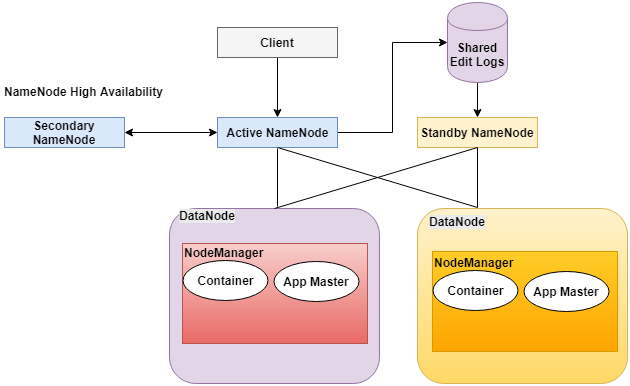
\includegraphics[width=\columnwidth]{images/HDFS_HA.png}
  \caption{HDFS High Availability Architecture}\label{f:hdfs-ha}
\end{figure}


\section{Conclusion}

Therefore, HDFS provides an efficient and reliable solution to process
large data files more efficiently while maintaining high availability
of data. By harnessing the power of multiple machines working in
parallel to split the large data into blocks, process the blocks
simultaneously and replicate the blocks into different racks, reading
and writing are faster as well the recovering from failure are much
shorter.

\bibliographystyle{ACM-Reference-Format}
\bibliography{report} 